\documentclass[10pt,landscape,letterpaper]{article}
\usepackage[utf8]{inputenc}
\usepackage[T1]{fontenc}
\usepackage{lmodern}
%\usepackage[LY1,T1]{fontenc}
%\usepackage{frutigernext}
%\usepackage[lf,minionint]{MinionPro}
\usepackage{tikz}
\usetikzlibrary{automata,shapes,positioning,arrows,fit,calc,graphs,graphs.standard}
\usepackage[nosf]{kpfonts}
\usepackage[t1]{sourcesanspro}
\usepackage{multicol}
\usepackage{wrapfig}
\usepackage[top=6mm,bottom=6mm,left=6mm,right=6mm]{geometry}
\usepackage[framemethod=tikz]{mdframed}
\usepackage{microtype}
\usepackage{pdfpages}
\usepackage[]{minted}
\usepackage{lipsum}
% https://tex.stackexchange.com/a/112573
\usepackage[most]{tcolorbox}
\usepackage{etoolbox}
\usepackage{listings}
\usepackage{realboxes}
\usetikzlibrary{arrows.meta}
\usepackage{enumitem} % allow to change list item separation
\usepackage{multirow}

% for easy SI units
\usepackage{siunitx}

\let\bar\overline

\definecolor{myblue}{cmyk}{1,.72,0,.38}

\def\firstcircle{(0,0) circle (1.5cm)}
\def\secondcircle{(0:2cm) circle (1.5cm)}

\colorlet{circle edge}{myblue}
\colorlet{circle area}{myblue!5}

\tikzset{filled/.style={fill=circle area, draw=circle edge, thick},
    outline/.style={draw=circle edge, thick}}
    
\pgfdeclarelayer{background}
\pgfsetlayers{background,main}

\everymath\expandafter{\the\everymath \color{myblue}}
\everydisplay\expandafter{\the\everydisplay \color{myblue}}

\renewcommand{\baselinestretch}{.8}
\pagestyle{empty}

% color for inline boxes
\definecolor{codegray}{rgb}{0.95,0.95,0.95}
\lstset{%
  basicstyle=\ttfamily,
  breaklines = true,
  backgroundcolor=\color{codegray},
}

% inline codeboxes
\definecolor{codegray}{rgb}{0.95,0.95,0.95}
\lstset{%1
  basicstyle=\ttfamily,
  breaklines = true,
  backgroundcolor=\color{codegray},
}
\newcommand*{\codebox}[1]{\Colorbox{codegray}{\lstinline|#1|}}

% short reverse to
\newcommand{\lrarr}{\longleftrightarrow}

\makeatletter % Author: https://tex.stackexchange.com/questions/218587/how-to-set-one-header-for-each-page-using-multicols
\renewcommand{\section}{\@startsection{section}{1}{0mm}%
                                {.2ex}%
                                {.2ex}%x
                                {\color{myblue}\sffamily\normalsize\bfseries}}
\renewcommand{\subsection}{\@startsection{subsection}{1}{0mm}%
                                {.2ex}%
                                {.2ex}%x
                                {\sffamily\bfseries}}

\makeatother
\setlength{\parindent}{0pt}

\begin{document}
%\footnotesize
\small
\begin{multicols*}{5}
  \section{Homework Examples}
\subsection{Utilization}
Using the topology in section \ref{ssec:delaytable} node A sends a file
of infinite size to node B. The packet size is \qty{1000}{\byte}. The
ACK is of negligible size so has 0 tranmission delay.

Using stop-and-wait for a single packet from $A\to R_1$ trans is \qty{1}{\milli\second} prop
is \qty{2}{\milli\second}, from $R_1\to R_2$ trans is
\qty{4}{\milli\second} prop is \qty{4}{\milli\second}, from $R_2\to B$
trans is \qty{1}{\milli\second} prop is \qty{2}{\milli\second}.

Total trans time is $1+4+1=6$ and total prop time is $2+4+2=8$. Total
time for ACK is just the prop time since it has negligible size. Total
time to wait for the ACK is $6+8\cdot2 = \qty{22}{\milli\second}$.

Utilization is at $A\to R_1$ transmission which is
\qty{1}{\milli\second}. Therefore, utilization is $\frac{1}{22}\approx
4.5\%$.

Now assume that we use Go-Back-N. There is no retrans timer the R nodes
have finite, but really large packet buffers. Links have no loses. What
is the max possible throughput without loses (remember that overflowing
the buffer will cause packet drop). We will use the bottleneck to
compute the sliding window. Total in flight time is
\qty{22}{\milli\second}. The bottleneck is at $R_1\to R_2$ and all that
matters is the transmisison delay which is \qty{4}{\milli\second}.
Therefore, sliding window can be of size
$\left\lceil\frac{22}{4}\right\rceil=6$ which is also the max \# of
in-flight packet.
\subsection{Routing Table Link State} \label{ssec:linkstateexp}
\resizebox{5cm}{!}{
\begin{tabular}{|r|r|r|r|r|}
  \hline
  \multicolumn{1}{|c|}{Step} &
  \multicolumn{1}{|c|}{N'} &
  $D(y), p(y)$ &
  $D(z), p(z)$ &
  $D(w), p(w)$ \\
  \hline
  \hline
  0 & $x$ & $\mathbf{4, x}$ & $\mathbf{50, x}$ & $\infty, \varnothing$ \\
  \hline
  1 & $xy$ & $4, x$ & $\mathbf{7, y}$ & $\mathbf{5, y}$ \\
  \hline
  2 & $xyw$ & $4, x$ & $\mathbf{6, w}$ & $5, y$ \\
  \hline
  3 & $xywz$ & $4, x$ & $6, w$ & $5, y$ \\
  \hline
\end{tabular}
}
Solution to
\begin{center}
  \resizebox{3cm}{!}{
  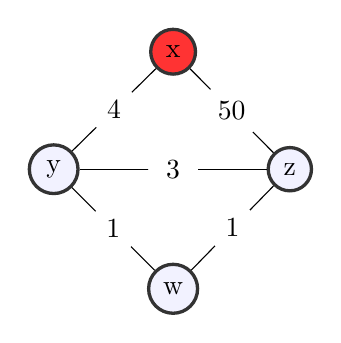
\begin{tikzpicture}[
    node distance=1.0cm,
    atnode/.style={
        circle, draw=black!80, fill=red!80, very thick, minimum size=2mm
      },
    visitnode/.style={
        circle, draw=black!80, fill=blue!40, very thick, minimum size=2mm
      },
    othernode/.style={
        circle, draw=black!80, fill=blue!5, very thick, minimum size=2mm
      },
    blanknode/.style={
        circle, draw=white, fill=white, very thick, minimum size=2mm
      },
    edgelbl/.style={
        circle, draw=white, fill=white
      },
  ]
  \node[blanknode](blank) {};
  \node[atnode](x) [above=of blank] {x};
  \node[othernode](y) [left=of blank] {y};
  \node[othernode](z) [right=of blank] {z};
  \node[othernode](w) [below=of blank] {w};

  % \path[-]
  %   (x) edge [above] node {4} (y)
  % ;
  \path[-, draw=black]
    (x) edge node[edgelbl] {$4$} (y)
    (x) edge node[edgelbl] {$50$} (z)
    (w) edge node[edgelbl] {$1$} (y)
    (w) edge node[edgelbl] {$1$} (z)
    (y) edge node[edgelbl] {$3$} (z)
  ;
  \end{tikzpicture}
  }
\end{center}
  \section{Quick Facts}
\subsection*{Miscellaneous Tips}
\footnotesize
\blockquote{A DNS server using UDP will query a different authoritative
server if its first query is lost (assuming there are multiple
authoritative servers). It attempts to maximize hit probability.}

\blockquote{A TCP handshake takes 1 RTT}

\blockquote{\textbf{Fast retransmission} requires 3 packets losses to be
triggered, and it halves the cwnd. \textbf{Slow retransmission} waits
for the recovery timer to expire and resets the cwnd}

\blockquote{\textbf{Stub resolver} must know the IP address of a caching
resolver. These are usually are the end users.}

\blockquote{\textbf{Cache resolvers} must know the IP address of a root
server.}

\blockquote{\textbf{Authoritative server} the final source of truth
(either address or CNAME).}

\small
\subsection*{Internet Protocol Stack}
\begin{itemize}
  \item \textbf{application}: DNS, FTP, SMTP, HTTP
  \item \textbf{transport}: TCP, UDP
  \item \textbf{network}: IP
  \item \textbf{link}: ethernet, WiFi
\end{itemize}
\subsection*{Stateless Protocols}
\begin{itemize}
  \item HTTP/1.1
  \item DNS
  \item UDP
\end{itemize}
\subsection*{Stateful Protocols}
\begin{itemize}
  \item TCP
\end{itemize}
\subsection*{Has re-trans. timers}
\begin{itemize}
  \item DNS caching resolver
  \item TCP data sender
\end{itemize}
\subsection*{DOESN'T have re-trans. Timers}
\begin{itemize}
  \item HTTP client/server
  \item DNS auth. server
  \item TCP data receiver
\end{itemize}
\subsection*{Common HTTP responses}
\begin{itemize}
  \item 200 OK: request succeeded
  \item 301 Moved Permanently: object moved to a location specified in the message
  \item 400 bad request: message not understood by server
  \item 505 HTTP version not supported
\end{itemize}
\subsection*{HTTP/1.0}
It uses TCP. Allows 1 request per connection. Each request needs to
reopen a connection. Allows parallel connections. Does not allow
pipelining
\subsection*{HTTP/1.1}
It uses TCP. Connection is persistent. As many requests per connection.
Allows pipelining and parallel connections.
\subsection*{HTTP/2.0}
Similar to HTTP/1.1 but it brakes down large packets into frames. This
allows to prevent some forms of head-of-line blocking (cannot prevent
inherent TCP HoL blocking). It also allows to send multiple streams of
data for multiplexing.
\subsection*{HTTP Packet Types}
\resizebox{5cm}{!}{
  \begin{tabular}{ |l|l|l|l|l|l|l| }
    \hline
    \multicolumn{1}{|c|}{Type} & \multicolumn{1}{|c|}{HTTP/1.0} & \multicolumn{1}{|c|}{HTTP/1.1} \\
    \hline
    GET    & yes      & yes \\
    \hline
    POST   & yes      & yes \\
    \hline
    HEAD   & yes      & yes \\
    \hline
    PUT    & no       & yes \\
    \hline
    DELETE & no       & yes \\
    \hline
  \end{tabular}
}
\subsection*{TCP + TLS}
\begin{center}
  \includegraphics[scale=0.4]{images/tcp-n-tls.png}
\end{center}
\subsection*{Go-Back-N}
Sender has sliding window and can send many unacknowledged packets.
Acknowledgement is for the latest received packet w/o error and sender
window slides. On packet loss it retransmits all packets in the sliding
window. ACKs are cumulative. It does not buffers packets.
\subsection*{Selective Repeat}
Sender has sliding window and can send many unacknowledged packets.
Receiver acknowledges each received packet, and it buffers them
(out-of-order if necessary). Sender "selects" ACKed packets and re-sends
unACKed ones when their individual timers expire.
  \section{Formulae}
\subsection*{ratios}
\begin{scriptsize}
P/E Ratio = Price Per Share / Earnings Per Share \\
Market to Book Ratio = Market Value per Share / Book Value per Share \\
Current Ratio = Current Assets/ Current Liabilities \\
Quick Ratio = (Current Assets - Inventory) / Current Liabilities \\
Cash Ratio = Cash / Current Liabilities \\
Debt/Equity = Total Debt / Total Equities \\
Total Debt Ratio = (Total Assets - Total Equity ) / Total Assets \\
\end{scriptsize}
\subsection*{others}
\begin{scriptsize}
Market Capitalization = Price per share $\times$ \# Shares Outstanding \\
Equity Multiplier = Total Assets / Total Equity \\
Times Interest Earned = (Earnings Before Interest And Taxes) / Interest \\
Cash Coverage = (EBIT + Depreciation + Amortization) / Interest \\
Inventory Turnover = Cost of Goods Sold / Inventory \\
Days' Sales in Inventory = 365 / (Inventory Turnover) \\
Receivables Turnover = Sales / Accounts Receivable \\
Days' Sales in Receivables = 365 / Receivables Turnover \\
Total Asset Turnover = Sales  /Total Assets  \\
Profit Margin = Net Income / Sales \\
Return on Assets = Net Income / Total Assets \\
Return on Equity = Net Income / Total Equity \\
EBITDA Margin = EBITDA / Sales \\
Capital Intensity = Total Assets / Sales \\
\end{scriptsize}

  \section{Terminology}
name server (NS), resource record (RR), content distribution network
(CDN), top level domains (TLDs), canonical name (CNAME), address (A),
transmission control protocol (TCP), user datagram protocol (UDP),
internet protocol (IP). maximum transmit unit (MTU). Don't fragment bit
(DF bit). More fragments bit (MF bit).
\end{multicols*}
\newpage
\begin{multicols*}{3}
  \section{Tables \& Diagrams}
\subsection{Congestion Control FSM}
\begingroup
\renewcommand{\arraystretch}{1.5} % Default value: 1
\begin{center}
  \resizebox{8cm}{!}{
    \begin{tabular}{|l|l|l|}
      \hline
      \multicolumn{3}{|c|}{\Large{Slow Start}}                                                     \\
      \hline
      Event Trigger                & Transition to                  & Action(s)                    \\
      \hline
      \hline
      \multirow{3}{*}{new ACK}     & \multirow{3}{*}{loop back}     & cwnd $\to$ cwnd + MSS        \\
      ~                            & ~                              & dupACK $\to$ 0               \\
      ~                            & ~                              & transmit new segments        \\
      \hline
      dupe ACK                     & loop back                      & dupACK++                     \\
      \hline
      cwnd $\geq$ ssthresh         & Congestion Avoidance           & do nothing                   \\
      \hline
      \multirow{4}{*}{timeout}     & \multirow{4}{*}{loop back}     & ssthresh $\to$ cwnd / 2      \\
      ~                            & ~                              & cwnd $\to$ 1 MSS             \\
      ~                            & ~                              & dupACK $\to$ 0               \\
      ~                            & ~                              & re-transmit missing segments \\
      \hline
      \multirow{3}{*}{dupACK == 3} & \multirow{3}{*}{Fast Recovery} & ssthresh $\to$ cwnd / 2      \\
      ~                            & ~                              & cwnd $\to$ ssthresh + 3 MSS  \\
      ~                            & ~                              & re-transmit missing segments \\
      \hline
    \end{tabular}
  }
\end{center}%
\begin{center}
  \resizebox{8cm}{!}{
    \begin{tabular}{|l|l|l|}
      \hline
      \multicolumn{3}{|c|}{\Large{Congestion Avoidance}}                                                 \\
      \hline
      Event Trigger                & Transition to                  & Action(s)                          \\
      \hline
      \hline
      \multirow{3}{*}{new ACK}     & \multirow{3}{*}{loop back}     & cwnd $\to$ cwnd + MSS (MSS / cwnd) \\
      ~                            & ~                              & dupACK $\to$ 0                     \\
      ~                            & ~                              & transmit new segments              \\
      \hline
      dupe ACK                     & loop back                      & dupACK++                           \\
      \hline
      \multirow{4}{*}{timeout}     & \multirow{4}{*}{Slow Start}    & ssthresh $\to$ cwnd / 2            \\
      ~                            & ~                              & cwnd $\to$ 1 MSS                   \\
      ~                            & ~                              & dupACK $\to$ 0                     \\
      ~                            & ~                              & re-transmit missing segments       \\
      \hline
      \multirow{3}{*}{dupACK == 3} & \multirow{3}{*}{Fast Recovery} & ssthresh $\to$ cwnd / 2            \\
      ~                            & ~                              & cwnd $\to$ ssthresh + 3 MSS        \\
      ~                            & ~                              & re-transmit missing segments       \\
      \hline
    \end{tabular}
  }
\end{center}%
\begin{center}
  \resizebox{8cm}{!}{
    \begin{tabular}{|l|l|l|}
      \hline
      \multicolumn{3}{|c|}{\Large{Fast Recovery}}                                                      \\
      \hline
      Event Trigger             & Transition to                         & Action(s)                    \\
      \hline
      \hline
      \multirow{2}{*}{new ACK}  & \multirow{2}{*}{Congestion Avoidance} & cwnd $\to$ ssthresh          \\
      ~                         & ~                                     & dupACK $\to$ 0               \\
      \hline
      \multirow{2}{*}{dupe ACK} & \multirow{2}{*}{loop back}            & cwnd $\to$ cwnd + MSS        \\
      ~                         & ~                                     & transmit new segments        \\
      \hline
      \multirow{4}{*}{timeout}  & \multirow{4}{*}{Slow Start}           & ssthresh $\to$ cwnd / 2      \\
      ~                         & ~                                     & cwnd $\to$ 1 MSS             \\
      ~                         & ~                                     & dupACK $\to$ 0               \\
      ~                         & ~                                     & re-transmit missing segments \\
      \hline
    \end{tabular}
  }
\end{center}
\endgroup
\subsection{Delay (tabulation)} \label{ssec:delaytable}
\begin{center}
  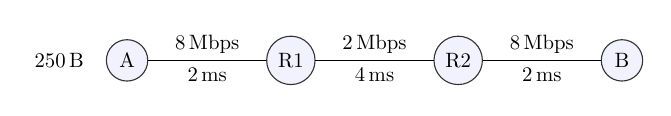
\begin{tikzpicture}[
    scale = 0.75, transform shape,
    >={Latex[black, length=1mm]},
    node distance=2cm,
    roundnode/.style={
        circle, draw=black!80, fill=blue!5, minimum size=7mm
      },
  ]
  \node[roundnode](A) {A};
  \node[roundnode](R1) [right=of A] {R1};
  \node[roundnode](R2) [right=of R1] {R2};
  \node[roundnode](B) [right=of R2] {B};
  \node[node distance=0.25cm] [left=of A] {\qty{250}{\byte}};
  \path[-]
    (A) edge [] node[above]{\qty{8}{Mbps}} (R1)
    (R1) edge [] node[above]{\qty{2}{Mbps}} (R2)
    (R2) edge [] node[above]{\qty{8}{Mbps}} (B)
    (A) edge [] node[below]{\qty{2}{ms}} (R1)
    (R1) edge [] node[below]{\qty{4}{ms}} (R2)
    (R2) edge [] node[below]{\qty{2}{ms}} (B)
  ;
  \end{tikzpicture}
  \begin{scriptsize}
    \begin{itemize}
      \item sending 4 packets from A to B
      \item In diagram propagation dealay is below link, and speed is above.
      \item base output delay is the transmission delay $\frac{\ell_\text{\tiny{pkt}}}{S_\text{\tiny{link}}}$ (use same units)
      \item base input delay is just the propagation delay.
    \end{itemize}
  \end{scriptsize}
  \resizebox{8cm}{!}{
    \begin{tabular}{ |r|r|r|r|r|r|r| }
      \hline
      \multicolumn{1}{|c|}{\textbf{src}} & \multicolumn{1}{c|}{speed} & \multicolumn{1}{c|}{prop} & \multicolumn{1}{c|}{speed} & \multicolumn{1}{c|}{prop} & \multicolumn{1}{c|}{speed} & \multicolumn{1}{c|}{prop} \\
      \hline
      \textbf{base} & 0.25ms & 2.00ms & 1.00ms & 4.00ms & 0.25ms & 2.00ms \\
      \hline
      \hline
      \multicolumn{1}{|c|}{P$_{\#}$} & \multicolumn{1}{c|}{A$\to$} & \multicolumn{1}{c|}{$\to$R1} & \multicolumn{1}{c|}{R1$\to$} & \multicolumn{1}{c|}{$\to$R2} & \multicolumn{1}{c|}{R2$\to$} & \multicolumn{1}{c|}{$\to$B} \\ [0.6ex]
      \hline
      1 & 0.25ms & 2.25ms & 3.25ms & 7.25ms & 7.50ms & 9.50ms \\
      \hline
      2 & 0.50ms & 2.50ms & 4.25ms & 8.25ms & 8.50ms & 10.50ms \\
      \hline
      3 & 0.75ms & 2.75ms & 5.25ms & 9.25ms & 9.50ms & 11.50ms \\
      \hline
      4 & 1.00ms & 3.00ms & 6.25ms & 10.25ms & 10.50ms & 12.50ms \\
      \hline
    \end{tabular}
  }
\end{center}
\begin{scriptsize}
  First fill the entire table using the base delay for each column. Now
  modify the table left to right and top to bottom without skipping
  columns. For every output column ($X\to$) take each term and add to it
  the max of the term to the left and above (use 0 if there is none).
  Then for every input column ($\to X$) simply add to each term the
  value of the column to the left.
\end{scriptsize}
\subsection{The Big Picture}
\begin{center}
  \resizebox{8cm}{!}{
  \includegraphics[]{images/big-picture.png}
  }
\end{center}
\end{multicols*}
\end{document}